% Lecture Template for ME3001-001-Tristan Hill - Spring 2017 - Fall 2017 - Fall 2020
% Mechanical Engineering Analysis with MATLAB
% Module 3 - Systems of Linear Equations 
% Topic 2 - Matrix Multiplication  

% !TEX TS-program = xelatex
% !TEX encoding = UTF-8 Unicode

% Spring 2020 - Summer 2020 - Fall 2020
% Tristan Hill, May 07, 2020 - June 12, 2020 - July 08, 2020
% Module Y - Sensors
% Topic 1 - Analog Sensors

\documentclass[fleqn]{beamer} % for presentation (has nav buttons at bottom)

\usepackage{/home/thill/Documents/lectures/mea_lectures/mea_lectures}


\newcommand{\MNUM}{3\hspace{2mm}} % Module number
\newcommand{\TNUM}{2\hspace{2mm}} % Topic number 
\newcommand{\moduletitle}{Systems of Linear Equations} % Titles and Stuff
\newcommand{\topictitle}{Matrix Multiplication} 

\newcommand{\sectiontitleI}{Motivation} % More Titles and Stuff
\newcommand{\sectiontitleII}{Multiplication of Conformible Matrices}
\newcommand{\sectiontitleIII}{Generalized Description of Multiplication}
\newcommand{\sectiontitleIV}{Exercise in MATLAB}


\author{ME3001 - Mechanical Engineering Analysis}
\title{Module \MNUM - \moduletitle}
\date{Mechanical Engineering\vspc Tennessee Technological University}

\begin{document}

\lstset{language=MATLAB,basicstyle=\ttfamily\small,showstringspaces=false}

\frame{\titlepage \center\begin{framed}\Large \textbf{Topic \TNUM - \topictitle}\end{framed} \vspace{5mm}}

% Section 0 - Outline
\frame{
	
	\large \textbf{Topic \TNUM - \topictitle} \vspace{3mm}\\
	
	\begin{itemize}
	
		\item \sectiontitleI    \vspc % Section I
		\item \sectiontitleII 	\vspc % Section II
		\item \sectiontitleIII 	\vspc %Section III
		\item \sectiontitleIV 	\vspc %Section IV
	
	\end{itemize}

}

\section{\sectiontitleI}

\frame{ 
  \frametitle{\sectiontitleI}
	\begin{itemize}
	\item Why do we need to multiply matrices? \vspace{20mm}\\
	
	\item Why do we need to use a computer?
	
	  
	  \end{itemize}
  
  }

\section{\sectiontitleII}

\frame{\small
  \frametitle{\sectiontitleII}
	
Consider 2 conformable matrices $F$ and $G$ with elements $f_{ij}$ and $g_{ij}$. Matrix Multiplication gives the product matrix $E$ with elements $e_{ij}$.\vspace{0mm} 
		 
		 \[E = F \times G \hspace{20mm} e_{ij}=\Sigma_{k=1}^n f_{ik}\times g_{kj}\] 
		 
	%	Here is an example with a two small matrices. \\
%\begin{fleqn}		 
		 \[
		  \left[ \begin{array}{cc}
e_{11} & e_{12}  \\
e_{21} & e_{22}  \end{array} \right]=	 	
 \left[ \begin{array}{ccc}
f_{11} & f_{12} & f_{13} \\
f_{21} & f_{22} & f_{23} \end{array} \right] \times \left[ \begin{array}{cc}
g_{11}&g_{12} \\
g_{21}&g_{22} \\
g_{31}&g_{32} \end{array} \right] 
		\]
%\end{fleqn}	

}

\section{\sectiontitleIII}

\frame{\small
  \frametitle{\sectiontitleIII}
\begin{fleqn}		 
\[ e_{ij}=\Sigma_{k=1}^n f_{ik}\times g_{kj} \]
	 
\[
		  \left[ \begin{array}{cc}
		e_{11} & e_{12}  \\
		& \\ 
		e_{21} & e_{22}  \end{array}	\right]=\left[ \begin{array}{c|c}
		f_{11}g_{11}+f_{12}g_{21}+f_{13}g_{31} & f_{11}g_{12}+f_{12}g_{22}+f_{13}g_{32}  \\
		& \\ 
		f_{21}g_{11}+f_{22}g_{21}+f_{23}g_{31} & f_{21}g_{12}+f_{22}g_{22}+f_{23}g_{32}  \end{array}	\right]
		 \]
		 
\end{fleqn}	
	
	
		\begin{itemize}
		
			\item What does that equation above mean? \\
			\item How can we write a {\it General Solution Technique} using the equation?
			
		\end{itemize}

}

\section{\sectiontitleIV}

\frame{\small
  \frametitle{\sectiontitleIII}
\textbf{A Programming Exercise - Matrix Multiplication}\\	
}

%\item \textbf{\LARGE What is Matrix Multiplication}	
%\begin{itemize}
%		\item Consider 2 conformable matrices $F$ and $G$ with elements $f_{ij}$ and $g_{ij}$. 
%		 \item Matrix Multiplication gives the product matrix $E$ with elements $e_{ij}$.  \\ \vspace{5mm}
%		 
%		 	 \scalebox{1.2}{ $E = F \times G \hspace{20mm} e_{ij}=\Sigma_{k=1}^n f_{ik}\times g_{kj}$} \\ \vspace{20mm}
%		 
%		 \item Lets do an example with a few small matrices. \\
%		 
%		 \scalebox{1.2}{$
%		  \left[ \begin{array}{cc}
%e_{11} & e_{12}  \\
%e_{21} & e_{22}  \end{array} \right]=	 	
% \left[ \begin{array}{ccc}
%f_{11} & f_{12} & f_{13} \\
%f_{21} & f_{22} & f_{23} \end{array} \right] \times \left[ \begin{array}{cc}
%g_{11}&g_{12} \\
%g_{21}&g_{22} \\
%g_{31}&g_{32} \end{array} \right] 
%$} 
%
%		 
%		 \vspace{20mm}
%		 
%		 \item A closer look at E \\ \vspace{10mm}
%		 
%\scalebox{1.2}{$
%		  \left[ \begin{array}{cc}
%		e_{11} & e_{12}  \\
%		& \\ 
%		e_{21} & e_{22}  \end{array}	\right]=\left[ \begin{array}{c|c}
%		f_{11}g_{11}+f_{12}g_{21}+f_{13}g_{31} & f_{11}g_{12}+f_{12}g_{22}+f_{13}g_{32}  \\
%		& \\ 
%		f_{21}g_{11}+f_{22}g_{21}+f_{23}g_{31} & f_{21}g_{12}+f_{22}g_{22}+f_{23}g_{32}  \end{array}	\right]
%		 $} \\\\
%		 
%	
%
%	\item So what is n ? 
%	\end{itemize}
%\newpage	
%	\item \textbf{\LARGE A Programming Exercise - Matrix Multiplication}\\	
%		\begin{itemize}
%		
%		\item  \scalebox{1.2}{ $e_{ij}=\Sigma_{k=1}^n f_{ik}\times g_{kj}$} \\
%		\item What does that equation mean? \\
%		\item How can we write a {\it General Solution Technique}?
%		\end{itemize}
%\newpage
%
%\item \textbf{\LARGE An Engineering Example - A Hanging Scaffolding}\\	
%		
%		As a group we are going to setup and solve a small statics problem. \\
%		
\includegraphics[scale=.75]{lecture2_fig1.png}\\
%		{\Large
%		\begin{itemize}
%		 \item \textbf{bar 1} 	\\\\
%		 \newpage
%		  \item \textbf{bar 2}	\\ \vspace{80 mm}
%		   \item \textbf{bar 3} 	\\\\
%		\end{itemize} }
%\newpage
%
%\item \textbf{\LARGE A Engineering Example (continued)}\\			
%
%\newpage
%\item \textbf{\LARGE An Engineering Example - A Simple Truss}\\\\	
%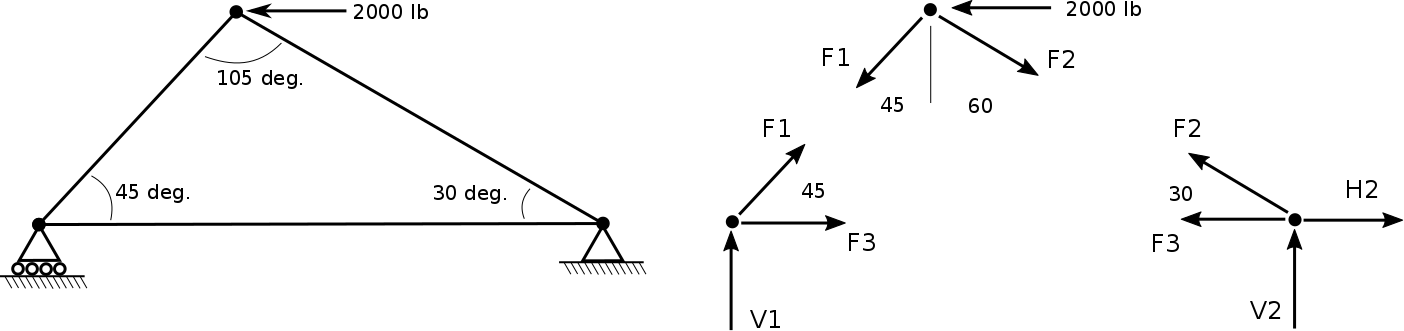
\includegraphics[scale=.30]{lecture2_fig2.png}
%		

		




%\newpage 
%
%	\item \textbf{ \LARGE REMINDER - Homework 2 has been Posted.} \\
%	 \item \textbf{ \LARGE REMINDER - Homework 2 is due Wed. Feb. 8} \\
%	\item \textbf{ \LARGE REMINDER - MATLAB script from today's lecture will be posted on ilearn. } \\
%
%\end{itemize}


	

\end{document}



